%!TEX encoding = UTF-8 Unicode
\documentclass{beamer}
\usepackage{amsmath,amsthm,amssymb}
\usepackage{CJKutf8}
\usepackage{graphicx}
\usepackage{hyperref}
\usepackage{pstricks-add}

\hypersetup{colorlinks,linkcolor=,unicode}
\useoutertheme{sidebar}
\usecolortheme{rose}
\usecolortheme{seahorse}
\newcommand{\Left} {\mathopen{}\mathclose\bgroup\left}
\newcommand{\Right}{\aftergroup\egroup\right}
\newcommand{\e}{\text e}
\newcommand{\ii}{\text i}
\newcommand{\NN}{\mathbb N}
\newcommand{\ZZ}{\mathbb Z}
\newcommand{\QQ}{\mathbb Q}
\newcommand{\RR}{\mathbb R}
\newcommand{\CC}{\mathbb C}
\renewcommand{\today}{\number\year~年~\number\month~月~\number\day~日}
\newcommand{\negskip}{\vskip -2em plus 3pt minus 3pt}

\theoremstyle{remark}
  \newtheorem{remark}{Remark}

\title{數值積分}
\author[何震邦]{何震邦 \href{mailto:jdh8@ms63.hinet.net}{\textless jdh8@ms63.hinet.net\textgreater}\\
    \href{http://creativecommons.org/licenses/by-sa/3.0/tw/deed.zh\textunderscore TW}{\includegraphics{by-sa.eps}}}

\begin{document}
\begin{CJK}{UTF8}{bsmi}
\maketitle

\section{黎曼和}
\begin{frame}{黎曼和}
  \begin{theorem}
    設 $[a,b]$ 分割為 $n$ 個子區間,每個區間的長度皆為 $h = \dfrac{b-a}{n}$。由左黎曼和得
    \[\int_a^b f(x)\,dx \approx h \sum_{k=0}^{n-1} f(x_k).\]
    由右黎曼和得
    \[\int_a^b f(x)\,dx \approx h \sum_{k=1}^{n} f(x_k).\]
  \end{theorem}
\end{frame}

\section{牛頓--寇次公式}
\begin{frame}{牛頓--寇次公式}
  \begin{theorem}
    若 $n \in \NN$,則
    \[\int_a^b f(x)\,dx \approx \sum_{k=0}^n w_k f \Left( a + \frac{k \left( b-a \right)}{n+1} \Right).\]
    $w_i$ 是由 $n$ 決定的常數。梯形法則和辛普森法則分別是 $n$ 為 1 和 2 的情況。
  \end{theorem}
\end{frame}

\subsection{梯形法則}
\begin{frame}{梯形法則}
  \begin{theorem}
    \[\int_a^b f(x)\,dx \approx \frac{b-a}{2} \left( f(a) + f(b) \right).\]
  \end{theorem}
  \begin{center}
    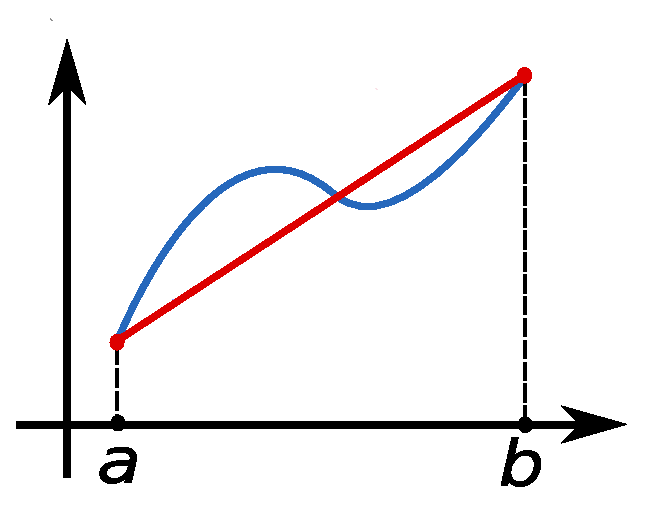
\includegraphics[width=0.5\textwidth]{Trapezoidal_rule_illustration}
  \end{center}
\end{frame}

\begin{frame}{分割區間後套用梯形法則}
  \begin{theorem}
    設 $[a,b]$ 分割為 $n$ 個子區間,每個區間的長度皆為 $h = \dfrac{b-a}{n}$。
    \begin{align*}
      \int_a^b f(x)\,dx &= \sum_{k=1}^{n} \int_{x_{k-1}}^{x_{k}} f(x)\,dx\\
	&\approx \frac{h}{2} \left( f(x_0) + 2 \sum_{k=1}^{n-1} f(x_{k}) + f(x_n) \right).
    \end{align*}
  \end{theorem}
\end{frame}

\subsection{辛普森法則}
\begin{frame}{辛普森法則}
  \begin{theorem}
    \[\int_a^b f(x)\,dx \approx \frac{b-a}{6} \left( f(a) + 4f \Left( \frac{a+b}{2} \Right) + f(b) \right).\]
  \end{theorem}
  \begin{center}
    \includegraphics[width=0.5\textwidth]{Simpsons_method_illustration}
  \end{center}
\end{frame}

\begin{frame}{分割區間後套用辛普森法則}
  \begin{theorem}
    設 $[a,b]$ 分割為 $n$ 個子區間,其中 $n$ 為偶數,每個區間的長度皆為 $h = \dfrac{b-a}{n}$。
    \begin{align*}
      &\:\int_a^b f(x)\,dx = \sum_{k=1}^{n/2} \int_{x_{2k - 2}}^{x_{2k}} f(x)\,dx\\
      \approx&\: \frac{h}{3} \left( f(x_0) + 2 \sum_{k=1}^{n/2 - 1} f(x_{2k}) + 4 \sum_{k=1}^{n/2} f(x_{2k - 1}) + f(x_n)
	  \right).
    \end{align*}
  \end{theorem}
\end{frame}

\begin{frame}
  \begin{center}
    \huge Thanks for your attention!
  \end{center}
\end{frame}
\end{CJK}
\end{document}
